
\begin{frame}
    \frametitle{Body biasing injection: LIRMM BBI platform}
%    Generateur
    \begin{textblock*}{40mm}(5mm, 25mm)
        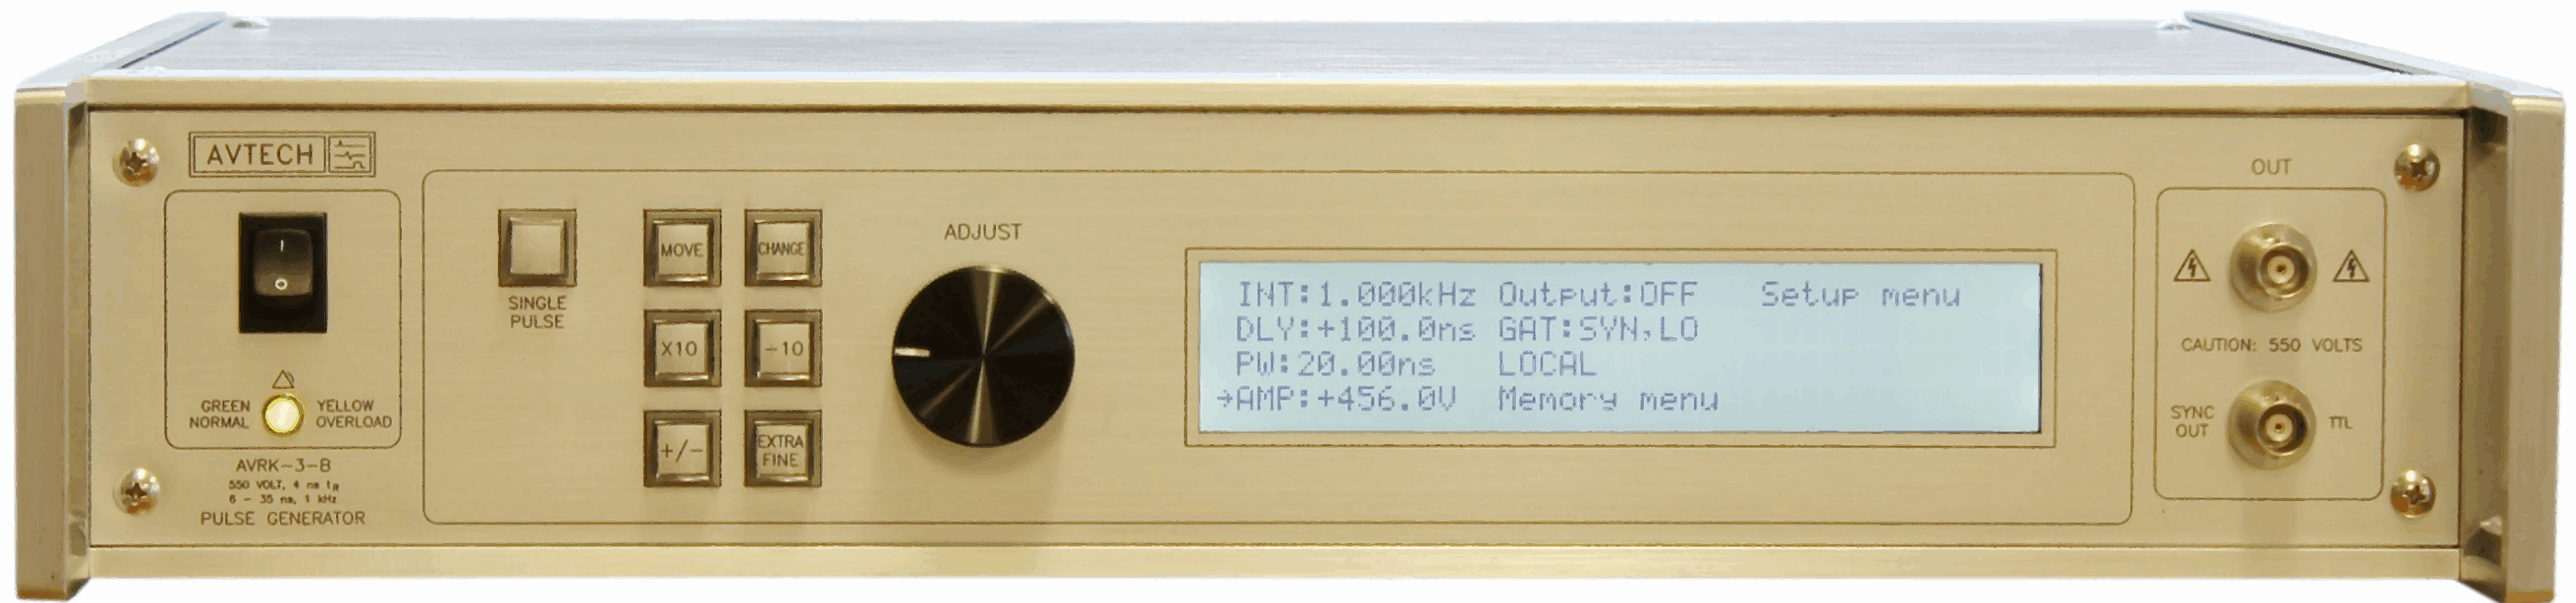
\includegraphics[width=\textwidth]{avrk4b.pdf}
    \end{textblock*}
%    Fleche generateur bas
    \begin{textblock*}{1mm}(24mm, 35mm)
        \begin{tikzpicture}
            \draw[-Latex, red, line width=0.5mm] (0, 0) -- (0, -1);
        \end{tikzpicture}
    \end{textblock*}
%    SOnde Loin
    \begin{textblock*}{30mm}(10mm, 47mm)
        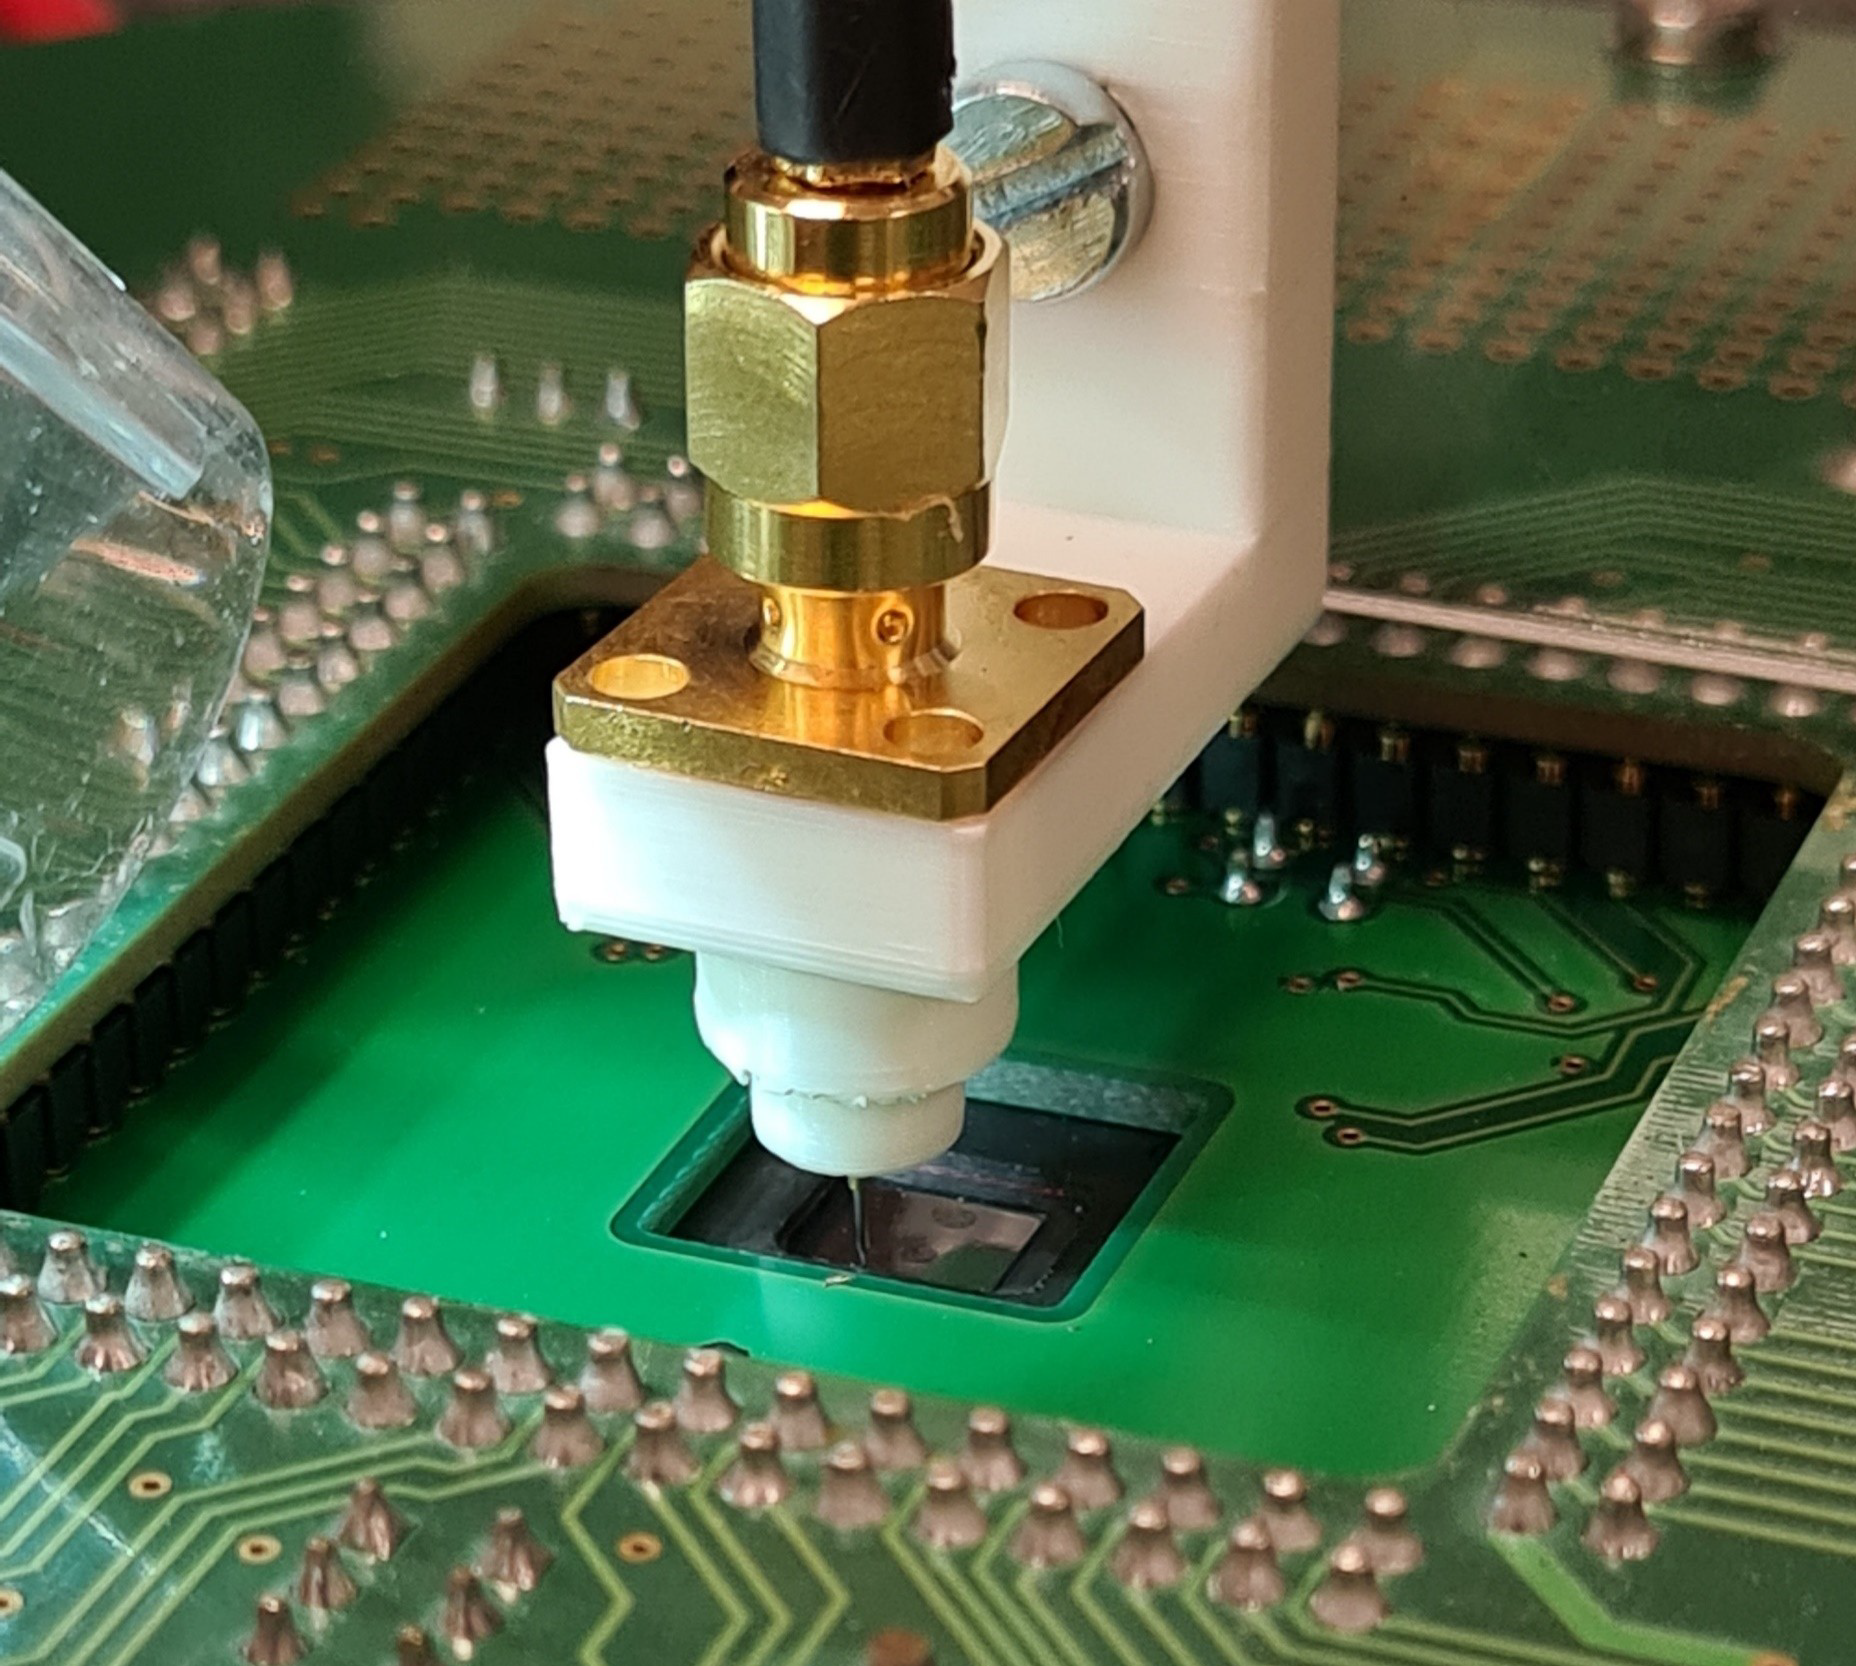
\includegraphics[width=\textwidth]{sondeBBI_loin_raw.png}
    \end{textblock*}
%    Fleche sonde loin droite
    \begin{textblock*}{1mm}(25.7mm, 68mm)
        \begin{tikzpicture}
            \draw[-Latex, red, line width=0.5mm] (0, 0) -- (1.8, -1);
        \end{tikzpicture}
    \end{textblock*}
%    Cercle sonde loin
    \begin{textblock*}{1mm}(21mm, 64mm)
        
\begin{tikzpicture}
            \draw[line width=0.5mm, color=red] circle (0.25);
        \end{tikzpicture}
    \end{textblock*}
%    SOnde proche
    \begin{textblock*}{30mm}(47mm, 64mm)
        \includegraphics[width=\textwidth]{pointeBBI2.png}
    \end{textblock*}
%    Header Tableau
    \begin{textblock*}{1mm}(85mm, 23mm)
        \textbf{\underline{Main platform characteristics:}}
    \end{textblock*}
%    Tableau
    \begin{textblock*}{1mm}(85mm, 26mm)
%        Main platform characteristics
        \begin{table}[]
            \begin{tabular}{|
                    >{\columncolor[HTML]{34CDF9}}c |
                    >{\columncolor[HTML]{FFFFFF}}c |}
                \hline
                & \\[-4mm]
                {\color[HTML]{000000} $V_{PULSE}$} & {\color[HTML]{000000} [150 ; 750] V} \\[1.1mm] \hline
                & \\[-4mm]
                $P_W$                              & [6 ; 20] ns                          \\[1.1mm] \hline
                & \\[-4mm]
                $T_R|T_F$                          & 4 ns                                 \\[1.1mm] \hline
                & \\[-4mm]
%                Recovery time                      & 1 ms                                 \\ \hline
                Propagation delay                  & $[150\cdot10^{-9} ; 1] \; s$         \\[1.1mm] \hline
                & \\[-4mm]
                Input jitter                       & $\pm \; 100 \; ps \pm 0.03 \%$       \\[1.1mm] \hline
                & \\[-4mm]
                Output coupling                    & DC                                   \\[1.1mm] \hline
                & \\[-4mm]
                $Gen. \; I_{MAX}$ (50 \textOmega)  & 16 A                                 \\[1.1mm] \hline
                & \\[-4mm]
%                $Probe \; I_{MAX}$                 & 3 A                                  \\ \hline
                Probe \diameter                    & 20 µm                                \\[1.1mm] \hline
            \end{tabular}
        \end{table}
    \end{textblock*}
%    Fleche generateur bas
    \begin{textblock*}{1mm}(72mm, 77.5mm)
        \begin{tikzpicture}
            \draw[-Latex, red, line width=0.5mm] (0, 0) -- (-1.25, 0.3);
        \end{tikzpicture}
    \end{textblock*}
\end{frame}

\section*{THESIS OBJECTIVES}
\begin{frame}
    \frametitle{Thesis objectives}
    \vspace{5mm}
    \Large
    \begin{itemize}
        \setlength\itemsep{1.5em}
        \item What is the spatial resolution of BBI?
        \item What is the time resolution of BBI?
        \item Is thinning the substrate useful in any way?
        \item How BBI induced faults occur?
        \item How to model BBI?
    \end{itemize}
\end{frame}

\section*{THESIS AGENDA}
\begin{frame}
    \frametitle{Thesis agenda}
    \vspace{5mm}
    \Large
    \begin{itemize}
        \setlength\itemsep{1.5em}
        \item Enhancing the practice of Body Biasing Injection
        \item Integrated circuits modeling for BBI
        \item Enhanced simulation flow
        \item Substrate thinning analysis in a BBI context
        \item Conclusion and outlooks
    \end{itemize}
\end{frame}
